% Options for packages loaded elsewhere
\PassOptionsToPackage{unicode}{hyperref}
\PassOptionsToPackage{hyphens}{url}
%
\documentclass[
]{article}
\usepackage{lmodern}
\usepackage{amssymb,amsmath}
\usepackage{ifxetex,ifluatex}
\ifnum 0\ifxetex 1\fi\ifluatex 1\fi=0 % if pdftex
  \usepackage[T1]{fontenc}
  \usepackage[utf8]{inputenc}
  \usepackage{textcomp} % provide euro and other symbols
\else % if luatex or xetex
  \usepackage{unicode-math}
  \defaultfontfeatures{Scale=MatchLowercase}
  \defaultfontfeatures[\rmfamily]{Ligatures=TeX,Scale=1}
\fi
% Use upquote if available, for straight quotes in verbatim environments
\IfFileExists{upquote.sty}{\usepackage{upquote}}{}
\IfFileExists{microtype.sty}{% use microtype if available
  \usepackage[]{microtype}
  \UseMicrotypeSet[protrusion]{basicmath} % disable protrusion for tt fonts
}{}
\makeatletter
\@ifundefined{KOMAClassName}{% if non-KOMA class
  \IfFileExists{parskip.sty}{%
    \usepackage{parskip}
  }{% else
    \setlength{\parindent}{0pt}
    \setlength{\parskip}{6pt plus 2pt minus 1pt}}
}{% if KOMA class
  \KOMAoptions{parskip=half}}
\makeatother
\usepackage{xcolor}
\IfFileExists{xurl.sty}{\usepackage{xurl}}{} % add URL line breaks if available
\IfFileExists{bookmark.sty}{\usepackage{bookmark}}{\usepackage{hyperref}}
\hypersetup{
  pdftitle={assignment},
  hidelinks,
  pdfcreator={LaTeX via pandoc}}
\urlstyle{same} % disable monospaced font for URLs
\usepackage[margin=1in]{geometry}
\usepackage{color}
\usepackage{fancyvrb}
\newcommand{\VerbBar}{|}
\newcommand{\VERB}{\Verb[commandchars=\\\{\}]}
\DefineVerbatimEnvironment{Highlighting}{Verbatim}{commandchars=\\\{\}}
% Add ',fontsize=\small' for more characters per line
\usepackage{framed}
\definecolor{shadecolor}{RGB}{248,248,248}
\newenvironment{Shaded}{\begin{snugshade}}{\end{snugshade}}
\newcommand{\AlertTok}[1]{\textcolor[rgb]{0.94,0.16,0.16}{#1}}
\newcommand{\AnnotationTok}[1]{\textcolor[rgb]{0.56,0.35,0.01}{\textbf{\textit{#1}}}}
\newcommand{\AttributeTok}[1]{\textcolor[rgb]{0.77,0.63,0.00}{#1}}
\newcommand{\BaseNTok}[1]{\textcolor[rgb]{0.00,0.00,0.81}{#1}}
\newcommand{\BuiltInTok}[1]{#1}
\newcommand{\CharTok}[1]{\textcolor[rgb]{0.31,0.60,0.02}{#1}}
\newcommand{\CommentTok}[1]{\textcolor[rgb]{0.56,0.35,0.01}{\textit{#1}}}
\newcommand{\CommentVarTok}[1]{\textcolor[rgb]{0.56,0.35,0.01}{\textbf{\textit{#1}}}}
\newcommand{\ConstantTok}[1]{\textcolor[rgb]{0.00,0.00,0.00}{#1}}
\newcommand{\ControlFlowTok}[1]{\textcolor[rgb]{0.13,0.29,0.53}{\textbf{#1}}}
\newcommand{\DataTypeTok}[1]{\textcolor[rgb]{0.13,0.29,0.53}{#1}}
\newcommand{\DecValTok}[1]{\textcolor[rgb]{0.00,0.00,0.81}{#1}}
\newcommand{\DocumentationTok}[1]{\textcolor[rgb]{0.56,0.35,0.01}{\textbf{\textit{#1}}}}
\newcommand{\ErrorTok}[1]{\textcolor[rgb]{0.64,0.00,0.00}{\textbf{#1}}}
\newcommand{\ExtensionTok}[1]{#1}
\newcommand{\FloatTok}[1]{\textcolor[rgb]{0.00,0.00,0.81}{#1}}
\newcommand{\FunctionTok}[1]{\textcolor[rgb]{0.00,0.00,0.00}{#1}}
\newcommand{\ImportTok}[1]{#1}
\newcommand{\InformationTok}[1]{\textcolor[rgb]{0.56,0.35,0.01}{\textbf{\textit{#1}}}}
\newcommand{\KeywordTok}[1]{\textcolor[rgb]{0.13,0.29,0.53}{\textbf{#1}}}
\newcommand{\NormalTok}[1]{#1}
\newcommand{\OperatorTok}[1]{\textcolor[rgb]{0.81,0.36,0.00}{\textbf{#1}}}
\newcommand{\OtherTok}[1]{\textcolor[rgb]{0.56,0.35,0.01}{#1}}
\newcommand{\PreprocessorTok}[1]{\textcolor[rgb]{0.56,0.35,0.01}{\textit{#1}}}
\newcommand{\RegionMarkerTok}[1]{#1}
\newcommand{\SpecialCharTok}[1]{\textcolor[rgb]{0.00,0.00,0.00}{#1}}
\newcommand{\SpecialStringTok}[1]{\textcolor[rgb]{0.31,0.60,0.02}{#1}}
\newcommand{\StringTok}[1]{\textcolor[rgb]{0.31,0.60,0.02}{#1}}
\newcommand{\VariableTok}[1]{\textcolor[rgb]{0.00,0.00,0.00}{#1}}
\newcommand{\VerbatimStringTok}[1]{\textcolor[rgb]{0.31,0.60,0.02}{#1}}
\newcommand{\WarningTok}[1]{\textcolor[rgb]{0.56,0.35,0.01}{\textbf{\textit{#1}}}}
\usepackage{graphicx,grffile}
\makeatletter
\def\maxwidth{\ifdim\Gin@nat@width>\linewidth\linewidth\else\Gin@nat@width\fi}
\def\maxheight{\ifdim\Gin@nat@height>\textheight\textheight\else\Gin@nat@height\fi}
\makeatother
% Scale images if necessary, so that they will not overflow the page
% margins by default, and it is still possible to overwrite the defaults
% using explicit options in \includegraphics[width, height, ...]{}
\setkeys{Gin}{width=\maxwidth,height=\maxheight,keepaspectratio}
% Set default figure placement to htbp
\makeatletter
\def\fps@figure{htbp}
\makeatother
\setlength{\emergencystretch}{3em} % prevent overfull lines
\providecommand{\tightlist}{%
  \setlength{\itemsep}{0pt}\setlength{\parskip}{0pt}}
\setcounter{secnumdepth}{-\maxdimen} % remove section numbering

\title{assignment}
\author{}
\date{\vspace{-2.5em}}

\begin{document}
\maketitle

\begin{Shaded}
\begin{Highlighting}[]
\NormalTok{stocks <-}\StringTok{ }\KeywordTok{read.csv}\NormalTok{(}\StringTok{"stocks.csv"}\NormalTok{)}
\KeywordTok{nrow}\NormalTok{(stocks)}
\end{Highlighting}
\end{Shaded}

\begin{verbatim}
## [1] 147
\end{verbatim}

\begin{Shaded}
\begin{Highlighting}[]
\KeywordTok{head}\NormalTok{(stocks)}
\end{Highlighting}
\end{Shaded}

\begin{verbatim}
##                                Name Symbol Market
## 1                   CDW Corporation    CDW    NDX
## 2                    VeriSign, Inc.   VRSN    NDX
## 3            Verisk Analytics, Inc.   VRSK    NDX
## 4 Microchip Technology Incorporated   MCHP    NDX
## 5                      JD.com, Inc.     JD    NDX
## 6                       Intuit Inc.   INTU    NDX
##                            Sector          Industry Market.cap..intra.day.
## 1 Information Technology Services        Technology                  16.46
## 2       Software鈥擨nfrastructure        Technology                  23.94
## 3             Consulting Services       Industrials                  30.37
## 4                  Semiconductors        Technology                  25.81
## 5                 Internet Retail Consumer Cyclical                  95.77
## 6          Software鈥擜pplication        Technology                  79.26
##   Enterprise.value Trailing.P.E Forward.P.E PEG.ratio..5.yr.expected.
## 1            20.19        22.53       18.54                      2.26
## 2            24.57        30.95       35.82                      3.86
## 3            33.57        63.92       35.86                      4.41
## 4            34.41        45.85       15.01                      1.98
## 5            91.58       423.74       31.30                     61.95
## 6            75.49        59.95       37.29                      4.19
##   Price.sales..ttm. Price.book..mrq. Enterprise.value.revenue
## 1              0.89            18.50                     1.09
## 2             19.22               NA                    19.72
## 3             11.37            14.62                    12.57
## 4              4.89             4.49                     6.53
## 5                NA             9.27                       NA
## 6             11.56            16.72                    11.01
##   Enterprise.value.EBITDA Total.ESG.risk.score Environmental.Risk.Score
## 1                   13.98                   11                        4
## 2                   28.46                   24                        3
## 3                   30.73                   21                        0
## 4                   18.04                   34                       16
## 5                      NA                   25                        7
## 6                   43.26                   18                        1
##   Social.Risk.Score Governance.Risk.Score
## 1                 3                     4
## 2                12                     8
## 3                15                     6
## 4                 9                     9
## 5                 9                     9
## 6                11                     6
\end{verbatim}

\begin{Shaded}
\begin{Highlighting}[]
\NormalTok{stocks <-}\StringTok{ }\KeywordTok{na.omit}\NormalTok{(stocks)}\OperatorTok
\StringTok{  }\KeywordTok{rename}\NormalTok{(}\DataTypeTok{intra_day=}\NormalTok{Market.cap..intra.day.)}\OperatorTok
\StringTok{  }\KeywordTok{rename}\NormalTok{(}\DataTypeTok{ent_value=}\NormalTok{Enterprise.value)}\OperatorTok
\StringTok{  }\KeywordTok{rename}\NormalTok{(}\DataTypeTok{trail_pe=}\NormalTok{Trailing.P.E)}\OperatorTok
\StringTok{  }\KeywordTok{rename}\NormalTok{(}\DataTypeTok{for_pe=}\NormalTok{Forward.P.E)}\OperatorTok
\StringTok{  }\KeywordTok{rename}\NormalTok{(}\DataTypeTok{peg=}\NormalTok{PEG.ratio..}\FloatTok{5.}\NormalTok{yr.expected.)}\OperatorTok
\StringTok{  }\KeywordTok{rename}\NormalTok{(}\DataTypeTok{ttm=}\NormalTok{Price.sales..ttm.)}\OperatorTok
\StringTok{  }\KeywordTok{rename}\NormalTok{(}\DataTypeTok{mrq=}\NormalTok{Price.book..mrq.)}\OperatorTok
\StringTok{  }\KeywordTok{rename}\NormalTok{(}\DataTypeTok{rev=}\NormalTok{Enterprise.value.revenue)}\OperatorTok
\StringTok{  }\KeywordTok{rename}\NormalTok{(}\DataTypeTok{ebitda=}\NormalTok{Enterprise.value.EBITDA)}
\CommentTok{#stocks <- na.omit(stocks)}
\CommentTok{#nrow(stocks)}
\end{Highlighting}
\end{Shaded}

147 variables with 102 having the missing value

\begin{Shaded}
\begin{Highlighting}[]
\KeywordTok{summary}\NormalTok{(stocks)}
\end{Highlighting}
\end{Shaded}

\begin{verbatim}
##      Name              Symbol             Market             Sector         
##  Length:45          Length:45          Length:45          Length:45         
##  Class :character   Class :character   Class :character   Class :character  
##  Mode  :character   Mode  :character   Mode  :character   Mode  :character  
##                                                                             
##                                                                             
##                                                                             
##    Industry           intra_day           ent_value            trail_pe     
##  Length:45          Min.   :      6.4   Min.   :      7.8   Min.   :  7.54  
##  Class :character   1st Qu.:     36.3   1st Qu.:     59.3   1st Qu.: 17.26  
##  Mode  :character   Median :     79.6   Median :    122.4   Median : 24.74  
##                     Mean   :  71455.7   Mean   :  70367.6   Mean   : 46.22  
##                     3rd Qu.:    204.8   3rd Qu.:    241.0   3rd Qu.: 41.50  
##                     Max.   :1670000.0   Max.   :1670000.0   Max.   :769.92  
##      for_pe           peg              ttm             mrq        
##  Min.   : 3.59   Min.   :-27.96   Min.   : 0.25   Min.   : 0.620  
##  1st Qu.:14.62   1st Qu.:  1.34   1st Qu.: 1.17   1st Qu.: 2.490  
##  Median :18.54   Median :  2.39   Median : 3.08   Median : 5.320  
##  Mean   :21.90   Mean   : 19.23   Mean   : 4.40   Mean   : 7.352  
##  3rd Qu.:25.85   3rd Qu.:  4.19   3rd Qu.: 5.94   3rd Qu.:11.710  
##  Max.   :98.25   Max.   :713.67   Max.   :18.62   Max.   :28.070  
##       rev             ebitda      Total.ESG.risk.score Environmental.Risk.Score
##  Min.   : 0.560   Min.   : 5.69   Min.   :11.00        Min.   : 0.000          
##  1st Qu.: 1.420   1st Qu.:11.48   1st Qu.:17.00        1st Qu.: 1.000          
##  Median : 3.670   Median :14.68   Median :20.00        Median : 2.000          
##  Mean   : 4.779   Mean   :18.52   Mean   :22.78        Mean   : 4.333          
##  3rd Qu.: 6.940   3rd Qu.:21.38   3rd Qu.:27.00        3rd Qu.: 7.000          
##  Max.   :17.570   Max.   :83.52   Max.   :40.00        Max.   :18.000          
##  Social.Risk.Score Governance.Risk.Score
##  Min.   : 3.00     Min.   : 4.0         
##  1st Qu.: 7.00     1st Qu.: 6.0         
##  Median :10.00     Median : 7.0         
##  Mean   :10.76     Mean   : 7.6         
##  3rd Qu.:14.00     3rd Qu.: 9.0         
##  Max.   :25.00     Max.   :12.0
\end{verbatim}

\begin{itemize}
\tightlist
\item
  Market capitalization refers to how much a company is worth as
  determined by the stock market. It is defined as the total market
  value of all outstanding shares. To calculate a company's market cap,
  multiply the number of outstanding shares by the current market value
  of one share. Companies are typically divided according to market
  capitalization: large-cap (\$10 billion or more), mid-cap (\$2 billion
  to \$10 billion), and small-cap (\$300 million to \$2 billion).
  Enterprise value includes in its calculation the market capitalization
  of a company but also short-term and long-term debt as well as any
  cash on the company's balance sheet. Enterprise value is used as the
  basis for many financial ratios that measure the performance of a
  company.
\item
  Enterprise value (EV) is a measure of a company's total value, often
  used as a more comprehensive alternative to equity market
  capitalization.
\item
  Trailing P/E is calculated by dividing the current market value, or
  share price, by the earnings per share over the previous 12 months.
\item
  The forward P/E ratio estimates a company's likely earnings per share
  for the next 12 months.
\item
  The PEG ratio enhances the P/E ratio by adding in expected earnings
  growth into the calculation. The PEG ratio is considered to be an
  indicator of a stock's true value, and similar to the P/E ratio, a
  \emph{lower PEG may indicate that a stock is undervalued}.
\item
  The P/S ratio is a key analysis and valuation tool that shows
  \emph{how much investors are willing to pay per dollar of sales for a
  stock.} The P/S ratio is typically calculated by dividing the stock
  price by the underlying company's sales per share.A low ratio could
  imply the stock is undervalued while a ratio that is
  higher-than-average could indicate that the stock is overvalued.
\item
  The P/B ratio measures the market's valuation of a company relative to
  its book value.\emph{The market value of equity is typically higher
  than the book value of a company.} P/B ratio is used by value
  investors to identify potential investments. P/B ratios under 1 are
  typically considered solid investments.
\item
  The enterprise value-to-revenue (EV/R) multiple helps compares a
  company's revenues to its enterprise value. \emph{The lower the
  better, in that, a lower EV/R multiple signals a company is
  undervalued.}
\item
  The enterprise value to earnings before interest, taxes, depreciation,
  and amortization ratio (EV/EBITDA) compares the value of a
  company---debt included---to the company's cash earnings less non-cash
  expenses. The EV/EBITDA metric is a popular valuation tool that helps
  investors compare companies in order to make an investment decision.
  EV calculates a company's total value or assessed worth, while EBITDA
  measures a company's overall financial performance and profitability.
  Typically, when evaluating a company, \emph{an EV/EBITDA value below
  10 is seen as healthy}. It's best to use the EV/EBITDA metric when
  comparing companies within the same industry or sector.
\end{itemize}

\begin{Shaded}
\begin{Highlighting}[]
\NormalTok{stocks }\OperatorTok\StringTok{ }
\StringTok{  }\NormalTok{dplyr}\OperatorTok{::}\KeywordTok{filter}\NormalTok{(ebitda}\OperatorTok{<}\DecValTok{10}\NormalTok{) }\OperatorTok\StringTok{ }
\StringTok{  }\KeywordTok{ggplot}\NormalTok{(}\KeywordTok{aes}\NormalTok{(ebitda, ebitda)) }\OperatorTok{+}\StringTok{ }
\StringTok{  }\KeywordTok{geom_boxplot}\NormalTok{() }\OperatorTok{+}\StringTok{ }
\StringTok{  }\KeywordTok{facet_wrap}\NormalTok{(}\OperatorTok{~}\NormalTok{Industry)}
\end{Highlighting}
\end{Shaded}

\includegraphics{ass2_files/figure-latex/unnamed-chunk-3-1.pdf}

\hypertarget{value-analysis}{%
\subsection{Value Analysis}\label{value-analysis}}

\begin{Shaded}
\begin{Highlighting}[]
\NormalTok{issuer<-stocks}\OperatorTok
\StringTok{  }\KeywordTok{select}\NormalTok{(Symbol,intra_day,ent_value,trail_pe,for_pe,peg,ttm,mrq,rev,ebitda)}

\NormalTok{pca_value<-issuer}\OperatorTok
\StringTok{  }\KeywordTok{select}\NormalTok{(intra_day,ent_value,trail_pe,for_pe,peg,ttm,mrq,rev,ebitda)}\OperatorTok
\StringTok{  }\KeywordTok{prcomp}\NormalTok{(}\DataTypeTok{scale.=}\OtherTok{TRUE}\NormalTok{)}
\KeywordTok{rownames}\NormalTok{(pca_value}\OperatorTok{$}\NormalTok{x)<-}\KeywordTok{pull}\NormalTok{(issuer,Symbol)}
\KeywordTok{biplot}\NormalTok{(pca_value, }\DataTypeTok{expand=}\DecValTok{10}\NormalTok{,}\DataTypeTok{xlim=}\KeywordTok{c}\NormalTok{(}\OperatorTok{-}\FloatTok{0.5}\NormalTok{,}\FloatTok{0.6}\NormalTok{),}\DataTypeTok{ylim=}\KeywordTok{c}\NormalTok{(}\OperatorTok{-}\FloatTok{0.05}\NormalTok{,}\FloatTok{0.1}\NormalTok{))}
\end{Highlighting}
\end{Shaded}

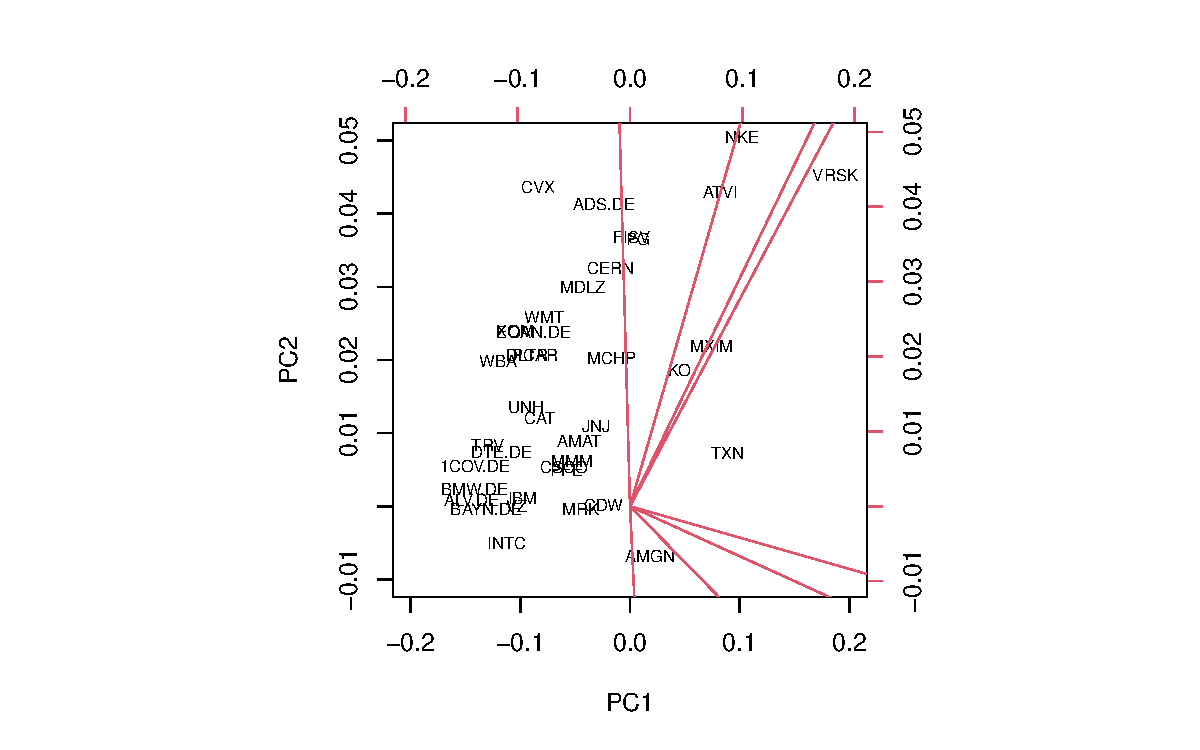
\includegraphics{ass2_files/figure-latex/value-1.pdf}

\begin{Shaded}
\begin{Highlighting}[]
\NormalTok{stocks }\OperatorTok\StringTok{ }\KeywordTok{filter}\NormalTok{(Industry }\OperatorTok{==}\StringTok{ "Technology"}\NormalTok{)}
\end{Highlighting}
\end{Shaded}

\begin{verbatim}
##                                           Name Symbol Market
## 1                              CDW Corporation    CDW    NDX
## 2            Microchip Technology Incorporated   MCHP    NDX
## 3                                  Intuit Inc.   INTU    NDX
## 4                                 Fiserv, Inc.   FISV    NDX
## 5              Maxim Integrated Products, Inc.   MXIM    NDX
## 6               Texas Instruments Incorporated    TXN    NDX
## 7                      Applied Materials, Inc.   AMAT    NDX
## 8                        Microsoft Corporation   MSFT    DJI
## 9                            Intel Corporation   INTC    DJI
## 10                         Cisco Systems, Inc.   CSCO    DJI
## 11                                  Apple Inc.   AAPL    DJI
## 12 International Business Machines Corporation    IBM    DJI
##                                 Sector   Industry  intra_day  ent_value
## 1      Information Technology Services Technology      16.46      20.19
## 2                       Semiconductors Technology      25.81      34.41
## 3               Software鈥擜pplication Technology      79.26      75.49
## 4      Information Technology Services Technology      67.25      90.64
## 5                       Semiconductors Technology      18.40      18.02
## 6                       Semiconductors Technology     118.06     122.41
## 7  Semiconductor Equipment & Materials Technology      59.04      59.32
## 8            Software鈥擨nfrastructure Technology 1540000.00 1490000.00
## 9                       Semiconductors Technology     204.10     216.97
## 10             Communication Equipment Technology     196.08     185.72
## 11                Consumer Electronics Technology 1670000.00 1670000.00
## 12     Information Technology Services Technology     109.12     167.26
##    trail_pe for_pe  peg   ttm   mrq   rev ebitda Total.ESG.risk.score
## 1     22.53  18.54 2.26  0.89 18.50  1.09  13.98                   11
## 2     45.85  15.01 1.98  4.89  4.49  6.53  18.04                   34
## 3     59.95  37.29 4.19 11.56 16.72 11.01  43.26                   18
## 4     56.21  18.81 1.32  5.40  2.13  7.28  22.63                   19
## 5     28.63  25.28 4.74  8.40 11.10  8.22  22.39                   24
## 6     24.20  23.65 2.55  8.62 15.44  8.94  19.45                   17
## 7     20.54  14.95 0.80  3.83  6.54  3.84  14.68                   15
## 8     35.40  27.78 2.11 10.79 13.05 10.42  22.66                   15
## 9      8.82  10.17 1.15  2.59  2.49  2.75   5.69                   15
## 10    18.41  14.74 2.42  3.88  5.49  3.67  11.48                   12
## 11    30.23  25.70 2.78  6.22 21.21  6.24  21.63                   24
## 12    13.94  10.07 4.40  1.45  5.32  2.21  10.94                   18
##    Environmental.Risk.Score Social.Risk.Score Governance.Risk.Score
## 1                         4                 3                     4
## 2                        16                 9                     9
## 3                         1                11                     6
## 4                         0                12                     7
## 5                         9                 7                     8
## 6                         6                 5                     6
## 7                         5                 4                     5
## 8                         0                 9                     5
## 9                         4                 5                     6
## 10                        1                 6                     6
## 11                        0                13                    10
## 12                        0                10                     7
\end{verbatim}

\hypertarget{risk}{%
\subsection{Risk}\label{risk}}

\begin{Shaded}
\begin{Highlighting}[]
\NormalTok{stocks }\OperatorTok\StringTok{ }\KeywordTok{select}\NormalTok{(Total.ESG.risk.score, Environmental.Risk.Score, Social.Risk.Score, Governance.Risk.Score)}
\end{Highlighting}
\end{Shaded}

\begin{verbatim}
##     Total.ESG.risk.score Environmental.Risk.Score Social.Risk.Score
## 1                     11                        4                 3
## 3                     21                        0                15
## 4                     34                       16                 9
## 6                     18                        1                11
## 7                     17                        0                10
## 8                     11                        1                 4
## 10                    31                        3                17
## 12                    19                        0                12
## 15                    20                        0                14
## 16                    20                        4                10
## 17                    24                        9                 7
## 19                    17                        6                 5
## 21                    35                        8                17
## 23                    26                       10                11
## 24                    15                        5                 4
## 29                    20                        0                13
## 30                    16                        0                 8
## 31                    15                        0                 9
## 32                    17                        2                 7
## 33                    15                        4                 5
## 34                    33                        1                20
## 35                    20                        2                12
## 36                    30                        2                16
## 38                    28                        4                18
## 39                    27                        2                14
## 40                    21                        0                15
## 41                    12                        1                 6
## 43                    26                        9                12
## 44                    22                        2                 9
## 45                    24                        0                13
## 46                    18                        3                11
## 48                    18                        0                10
## 50                    17                        0                10
## 52                    35                       13                14
## 54                    37                        7                20
## 56                    40                       18                12
## 57                    32                       16                 9
## 85                    24                        8                10
## 87                    17                        2                 7
## 96                    38                        3                25
## 97                    14                        2                 4
## 99                    27                        7                 8
## 105                   17                        1                 6
## 140                   20                       11                 3
## 147                   26                        8                 9
##     Governance.Risk.Score
## 1                       4
## 3                       6
## 4                       9
## 6                       6
## 7                       6
## 8                       6
## 10                     11
## 12                      7
## 15                      7
## 16                      6
## 17                      8
## 19                      6
## 21                      9
## 23                      6
## 24                      5
## 29                      7
## 30                      8
## 31                      5
## 32                      8
## 33                      6
## 34                     11
## 35                      6
## 36                     12
## 38                      7
## 39                     11
## 40                      6
## 41                      6
## 43                      5
## 44                     11
## 45                     10
## 46                      4
## 48                      7
## 50                      7
## 52                      8
## 54                     10
## 56                     10
## 57                      8
## 85                      6
## 87                      7
## 96                     11
## 97                      7
## 99                     12
## 105                    10
## 140                     6
## 147                     8
\end{verbatim}

\begin{Shaded}
\begin{Highlighting}[]
\NormalTok{d <-}\StringTok{ }\KeywordTok{apply}\NormalTok{(}\KeywordTok{cbind}\NormalTok{(stocks}\OperatorTok{$}\NormalTok{Environmental.Risk.Score, stocks}\OperatorTok{$}\NormalTok{Social.Risk.Score, stocks}\OperatorTok{$}\NormalTok{Governance.Risk.Score), }\DecValTok{1}\NormalTok{, sum)}
\end{Highlighting}
\end{Shaded}

\begin{Shaded}
\begin{Highlighting}[]
\KeywordTok{all}\NormalTok{(stocks}\OperatorTok{$}\NormalTok{Total.ESG.risk.score }\OperatorTok{==}\StringTok{ }\NormalTok{d)}
\end{Highlighting}
\end{Shaded}

\begin{verbatim}
## [1] FALSE
\end{verbatim}

\begin{Shaded}
\begin{Highlighting}[]
\CommentTok{# checking if total esg risk score = environmrnt + social + government }
\NormalTok{stocks_tesg <-}\StringTok{ }\NormalTok{stocks[stocks[,}\DecValTok{15}\NormalTok{] }\OperatorTok{==}\StringTok{ }\NormalTok{d,]}
\NormalTok{d <-}\StringTok{ }\KeywordTok{apply}\NormalTok{(}\KeywordTok{cbind}\NormalTok{(stocks_tesg}\OperatorTok{$}\NormalTok{Environmental.Risk.Score, stocks_tesg}\OperatorTok{$}\NormalTok{Social.Risk.Score, stocks_tesg}\OperatorTok{$}\NormalTok{Governance.Risk.Score), }\DecValTok{1}\NormalTok{, sum)}
\KeywordTok{all}\NormalTok{(stocks_tesg}\OperatorTok{$}\NormalTok{Total.ESG.risk.score }\OperatorTok{==}\StringTok{ }\NormalTok{d, }\DataTypeTok{na.rm =} \OtherTok{TRUE}\NormalTok{)}
\end{Highlighting}
\end{Shaded}

\begin{verbatim}
## [1] TRUE
\end{verbatim}

\begin{Shaded}
\begin{Highlighting}[]
\NormalTok{stocks_risk <-}\StringTok{ }\NormalTok{stocks_tesg }\OperatorTok\StringTok{ }\KeywordTok{select}\NormalTok{(Symbol, Environmental.Risk.Score, Social.Risk.Score, Governance.Risk.Score)}
\NormalTok{stocks_risk <-}\StringTok{ }\KeywordTok{na.omit}\NormalTok{(stocks_risk)}
\end{Highlighting}
\end{Shaded}

\begin{Shaded}
\begin{Highlighting}[]
\NormalTok{pca_risk <-}\StringTok{ }\NormalTok{stocks_risk }\OperatorTok\StringTok{ }\KeywordTok{select_if}\NormalTok{(is.numeric) }\OperatorTok\StringTok{ }\KeywordTok{prcomp}\NormalTok{(}\DataTypeTok{scale. =} \OtherTok{TRUE}\NormalTok{)}
\KeywordTok{rownames}\NormalTok{(pca_risk}\OperatorTok{$}\NormalTok{x) <-}\StringTok{ }\KeywordTok{pull}\NormalTok{(stocks_risk, Symbol)}
\KeywordTok{biplot}\NormalTok{(pca_risk, }\DataTypeTok{xlim=}\KeywordTok{c}\NormalTok{(}\OperatorTok{-}\FloatTok{0.35}\NormalTok{,}\FloatTok{0.25}\NormalTok{), }\DataTypeTok{cex=}\FloatTok{0.7}\NormalTok{)}
\end{Highlighting}
\end{Shaded}

\includegraphics{ass2_files/figure-latex/pca_risk-1.pdf}

\end{document}
